\documentclass[11pt]{article}
\usepackage{moreverb}    % Defines {listing} environment.
\usepackage{tocloft}
\usepackage{geometry}            % See geometry.pdf to learn the layout options. There are lots.
\usepackage{xspace}
\geometry{letterpaper}           % ... or a4paper or a5paper or ... 
%\usepackage[parfill]{parskip}   % To begin paragraphs with an empty line rather than an indent
\usepackage{graphicx}
\usepackage{amssymb}
\usepackage{amsmath}
\usepackage{alltt}
\usepackage[T1]{fontenc}   % so _, <, and > print correctly in text.
\usepackage[strings]{underscore}    % to use "_" in text
\usepackage[pdftex,colorlinks=true,bookmarksnumbered=true]{hyperref}

\newcommand{\fig}[1]{Figure~\ref{#1}}
\newcommand{\lux}{Lux\xspace}
\newcommand{\chess}{CHESS\xspace}
\newcommand{\Begineq}{\begin{equation}}
\newcommand{\Endeq}{\end{equation}}
\newcommand{\CRNO}{\nonumber \\}
\newcommand{\Eq}[1]{{Eq.~(\protect\ref{#1})}}
\newcommand\ttcmd{\begingroup\catcode`\_=11 \catcode`\%=11 \dottcmd}  % Must be last package!
\newcommand\dottcmd[1]{\texttt{#1}\endgroup}
\newcommand{\vn}{\ttcmd}   

\newcommand{\Newline}{\hfil \\}
\newcommand{\sref}[1]{$\S$\ref{#1}}

\newenvironment{example}
  {\vspace{\ExBeg} \begin{alltt}}
  {\end{alltt} \vspace{\ExEnd}}

%---------------------------------------------------------------------------------

\newlength{\dPar}
\newlength{\ExBeg}
\newlength{\ExEnd}
\setlength{\dPar}{1.5ex}
\setlength{\ExBeg}{-\dPar}
\addtolength{\ExBeg}{-0.5ex}
\setlength{\ExEnd}{-\dPar}
\addtolength{\ExEnd}{-0.0ex}

\setlength{\textwidth}{6.25in}
\setlength{\hoffset}{0.0in}
\setlength{\oddsidemargin}{0.25in}
\setlength{\evensidemargin}{0.0in}
\setlength{\textheight}{8.5in}
\setlength{\topmargin}{0in}

\setlength{\parskip}{\dPar}
\setlength{\parindent}{0ex}

\setlength\cftparskip{0pt}
\setlength\cftbeforesecskip{3pt}
\setlength\cftaftertoctitleskip{15pt}

%---------------------------------------------------------------------------------

\title{Lux Program}
\author{D. Sagan, K. Finkelstein}
\date{June 3, 2022}

%---------------------------------------------------------------------------------

\begin{document}
\maketitle

\pdfbookmark[1]{Contents}{Contents}
\tableofcontents

%------------------------------------------------------------------
\section{Introduction} 
\label{s:intro}

\lux is a program for Monte Carlo simulations of X-rays using either coherent or incoherent ray
tracing. \lux works by generating photons at a source element and tracking them through to a
detector. \lux uses the Bmad subroutine library\cite{b:bmad} for tracking and lattice bookkeeping.

\lux comes in two versions: A single threaded version whose executable is called \vn{lux} and an
parallel compute version using MPI whose executable is called \vn{lux_mpi}. [Note to Distribution
maintainers: The single threaded version will always be built when compiling the Distribution. The
MPI version is built by building the Distribution with MPI enabled. See the documentation on the
Bmad web site for more details.]

%------------------------------------------------------------------
\section{Running \lux} 
\label{s:run}

See the documentation for setting up the Bmad environment variables at
\begin{example}
  \url{https://wiki.classe.cornell.edu/ACC/ACL/RunningPrograms}
\end{example}

Once the Bmad environment variables have bee set, the syntax for invoking the single threaded
version of \lux is
\begin{example}
  lux \{-silent\} \{<master-input-file-name>\}
\end{example}
The \vn{<master-input-file-name>} optional argument is used to set the master input file name. The
default is ``\vn{lux.init}''.

The \vn{-silent} optional argument suppresses the terminal output that \lux generates at the end of
a run. This is useful to avoid long output when \lux is run repeatedly via a script.

Example input files are in the \vn{\$ACC_ROOT_DIR/lux/examples} subdirectory.

To run the parallel version of \lux, see the documentation on running programs on the Bmad web site
for more details. If running on a single machine (as opposed to multiple machines in a cluster),
typically \vn{mpirun} or \vn{mpiexec} is used. Example:
\begin{example}
  mpirun -np 8 lux_mpi
\end{example}

Note that two input files are always required to run \lux: The master input file
(\sref{s:master.file}) and the Bmad lattice file (\sref{s:lat.file}).

%------------------------------------------------------------------
\section{Fortran Namelist}
\label{s:namelist}

Fortran namelist syntax is used for setting parameters in \lux's
master input file (\sref{s:master.file}). The general form of a
namelist is
\begin{example}
  &<namelist_name>
    <var1> = ...
    <var2> = ...
    ...
  /
\end{example}
The tag \vn{"\&<namelist_name>"} starts the namelist where
\vn{<namelist_name>} is the name of the namelist. The namelist ends
with the slash \vn{"/"} tag. Anything outside of this is
ignored. Within the namelist, an exclamation mark \vn{"!"} and
everything after it on a line is ignored. \vn{<var1>}, \vn{<var2>},
etc. are variable names. Example:
\begin{example}
  &section_def section =   0.0, "arc_std", "elliptical", 0.045, 0.025 /
\end{example}
here \vn{section_def} is the namelist name and \vn{section} is a variable
name.  Notice that here \vn{section} is a ``structure'' which has five
components (0.0, ``arc_str'', etc.).



%------------------------------------------------------------------
\section{Master Input File} 
\label{s:master.file}

%------------------------------------------------------------------
\subsection{Master Input File Example}
\label{ss:master.example}

The master input file consists of a single \vn{namelist} called \vn{params}.
An example is:
\begin{example}
  &params
    lux_param%lattice_file = "test.bmad"         ! Defines experimental layout.
    lux_param%det_pix_out_file = "lux.det_pix#"
    lux_param%photon1_out_file = "lux.photon1"   ! Individual photon positions.
    lux_param%track_out_file = "track.dat"       ! Element-by-element track info.
    lux_param%bmad_parameters_out = ""           ! Parameters to include in 
                                                 !             det_pix_out_file.
    lux_param%photon_init_element = "p_init"     ! Name of element emitting photons
    lux_param%detector_element = "det"
    lux_param%photon1_element = ""

    lux_param%random_seed = 0                    ! 0 => Use system clock
    lux_param%random_engine = "pseudo"

    lux_param%scale_initial_field_to_1 = False
    lux_param%intensity_normalization_coef = 1e6 ! photon intensities norm.
    lux_param%normalization_includes_pixel_area = T

    lux_param%stop_total_intensity = 10          ! Cumulative intensity to stop at.
    lux_param%stop_num_photons = 1e8             ! Max number of photons to track.
    lux_param%mpi_run_size = 0.1                 ! Normalized num photons to track.

    lux_param%intensity_min_det_pixel_cutoff = 0.1 ! det_pix_out file Cutoff

    lux_param%intensity_min_photon1_cutoff = 1e-3  ! photon1_out file cutoff
    lux_param%n_photon1_out_max = 100              ! Max photons in photon1_out_file.
    lux_param%reject_dead_at_det_photon1 = False
    lux_param%timer_print_dtime = 300

    lux_param%histogram_variable = "x_angle"     ! Histogram independent var.
    lux_param%histogram_bin_width = 1e-4         ! Width of histogram bins.
  /
\end{example}

%------------------------------------------------------------------
\subsection{Master Input File Parameters}
\label{ss:master.params}

The following is a complete list of the components of the params namelist:
  \begin{description}
  \item[\vn{lux_param\%bmad_parameters_out}] \Newline
Semicolon delimited list of parameters from the Bmad lattice file to include in the
\vn{det_pix_out_file} header. This header records the values of various parameters and this can be
used in post processing. For example, for the example Bmad lattice shown in
Section~\sref{ss:x.ray.init}, \vn{lux_param%bmad_parameters_out} could be set to:
\begin{example}
  lux_param%bmad_parameters_out = "angle;cryst[graze_angle_in]"
\end{example}
In this case there are two parameters to be recorded in the \vn{det_pix_out_file}: The parameter
called \vn{angle} and the parameter \vn{cryst[graze_angle_in]}. This latter parameter is the
\vn{graze_angle_in} parameter of the \vn{cryst} lattice element. In the \vn{det_pix_out_file}
header, \lux would put the values of these two parameters:
\begin{example}
  angle = 1.396263
  cryst__graze_angle_in = 0.12634
\end{example}
Notice that the name used for the \vn{cryst[graze_angle_in]} parameters has been mangled to make it
readable by a python script. In particular, the ``['' character is replaced by ``\_\_'' and the ``]''
character is removed.
  %
  \item[\vn{lux_param\%det_pix_out_file}] \Newline
Name of the output data file recording the X-ray intensity on the
detector. See section~\sref{s:det.pix.file} for more details. The file
name may be ``numbered'' using a ``\#'' character (\sref{s:number}). A
blank file name will prevent a file being generated.
  %
  \item[\vn{lux_param\%detector_element}] \Newline
Name of the lattice detector element where the photon are absorbed.
  %
  \item[\vn{lux_param\%histogram_bin_width}] \Newline
Bin width of histogram. See \sref{s:histo.file} for more details.
  %
  \item[\vn{lux_param\%histogram_variable}] \Newline
Variable used in constructing the histogram (\sref{s:histo.file}).
Possibilities are:
\begin{example}
  "init_x"        ! Initial photon x-position.
  "init_y"        ! Initial photon y-position.
  "init_x_angle"  ! Initial angle of photon velocity in the (z,x) plane.
  "init_y_angle"  ! Initial angle of photon velocity in the (z,y) plane.
  "x_angle"       ! Angle of photon velocity in then (z,x) plane at the detector.
  "y_angle"       ! Angle of photon velocity in the (z,y) plane at the detector.
  "energy"        ! photon energy relative to the reference (default).
\end{example}
If not given then no histogram file is produced.
  %
  \item[\vn{lux_param\%intensity_min_det_pixel_cutoff}] \Newline
Sets the threshold absorbed photon intensity such that all pixels
who's intensity is below this will not be included in the
\vn{det_pix_out} file (\sref{s:det.pix.file}). This intensity is
relative to the maximum pixel intensity.
  %
  \item[\vn{lux_param\%intensity_min_photon1_cutoff}] \Newline
Cutoff intensity below which a photon will not be included in
the photon1_out file (\sref{s:photon1.file}).
  %
  \item[\vn{lux_param\%intensity_normalization_coef}] \Newline
Coefficient used to normalize the photon intensity with (\sref{s:photon.descrip}).
  %
  \item[\vn{lux_param\%lattice_file}] \Newline
Name of the input file that defines the X-ray optics setup from source
to detector. The syntax of the file conforms to the Bmad lattice
format. The Bmad manual has a detailed description of this format.
Examples are presented in section~\sref{s:lat.file}.
  %
  \item[\vn{lux_param\%mpi_run_size}] \Newline
Only used when running the parallel version of \lux. This parameter
determines how many photons a slave process is asked to track before
sending back data to the master process:
\begin{example}
  Number to track = lux_param%stop_num_photons * 
           lux_param%mpi_run_size / (Number_processes - 1)
\end{example}
\vn{%mpi_run_size} should be set to some number between 0 and 1.
The value 0.1 is the default. Changing this number can affect
running time but the running time should be fairly insensitive
to the value of \vn{%mpi_run_size}.
  %
  \item[\vn{lux_param\%normalization_includes_pixel_area}] \Newline
Does the factor used for computing the normalized photon intensity (\sref{s:photon.descrip}) include
the pixel area of the detector?
  %
  \item[\vn{lux_param\%photon_init_element}] \Newline
Name of the lattice element that is the source of the photons (\sref{s:lat.file}).
  %
  \item[\vn{lux_param\%n_photon1_out_max}] \Newline
Maximum number of photons to record in the \vn{photon1_out_file}.
Default is 100.
  %
  \item[\vn{lux_param\%photon1_element}] \Newline
The photon position values in the photon1_out file will be the
photon position at the lattice element named by \vn{lux_param%photon1_element}. 
If \vn{photon1_element} is blank (default), the
detector element used will be used (\sref{s:photon1.file}).
  %
  \item[\vn{lux_param\%photon1_out_file}] \Newline
Name of the output data file recording the starting and ending
positions of individual photons. See section~\sref{s:photon1.file} for
more details. The file name may be ``numbered'' using 
a ``\#'' character (\sref{s:number}). A blank file name will prevent a
file being generated.
  %
  \item[\vn{lux_param\%random_engine}] \Newline
Type of ``random'' number generator to use. Possibilities are:
\begin{example}
  quasi      
  pseudo      ! Default
\end{example}
The \vn{quasi} number generator gives a more-or-less uniform
distribution of numbers. That is, a quasi random generator is not
actually random. The numbers generated with the quasi random generator
are always the same from run to run.
  %
  \item[\vn{lux_param\%random_seed}] \Newline
If the \vn{random_engine} is set to \vn{pseudo}, \vn{%random_seed} is the random number seed used by
the random number generator. If set to 0, the system clock will be used so that the output results
will show statistical variations from run to run. Not used if the \vn{random_engine} is set to
\vn{quasi}.  If the seed is nonzero, the results will be the same from run to run. However, the
results when using the MPI version of \lux will not be exactly the same at the non-MPI \lux version.
  %
  \item[\vn{lux_param\%reject_dead_at_det_photon1}] \Newline
If \vn{reject_dead_to_det_photon1} is set to True, do not print to the photon_out file any photons
that do not reach the detector. This switch is only relevant when the lattice element at which the
photon positions are being evaluated is not the detector (\sref{s:photon1.file}).
  %
  \item[\vn{lux_param\%scale_initial_field_to_1}] \Newline
Scale the field so that $E_x^2 + E_y^2 = 1$? Default is True. Only used if at least one field
component is non-zero. See \sref{s:photon.descrip} for more details.
  %
  \item[\vn{lux_param\%stop_num_photons}] \Newline
Maximum number of photons to track (\sref{s:det}).
  %
  \item[\vn{lux_param\%stop_total_intensity}] \Newline
Cumulative unnormalized intensity at the detector to stop
at (\sref{s:det}).  Note: This parameter is ignored if running the
parallel version of \lux and only \vn{lux_param%stop_num_photons}
is used.
  %
  \item[\vn{lux_param\%timer_print_dtime}] \Newline
The program will print a tracking status message every so often. The nominal time between status
messages is set by \vn{lux_param%timer_print_dtime} which is a number in seconds. The default is
\vn{300}.
  %
  \item[\vn{lux_param\%track_out_file}] \Newline
The \vn{track_out_file} records how many photons are lost at each lattice element. This is useful for
diagnosing cases when too many photons are being lost before reaching the detector.
  \end{description}

%------------------------------------------------------------------
\section{Lattice Description File}
\label{s:lat.file}

The name of the lattice description file which defines the
experimental setup is given by the \vn{lattice_file} parameter in the
master input file (\sref{s:master.file}). Bmad standard syntax is
used\cite{b:bmad}. 

The starting element for tracking photons, specified by the
\vn{lux_param%photon_init_element} parameter must be of type:
\begin{example}
  photon_init
\end{example}
This element may have an associated ``physical source'' element which
should be a bend, wiggler, or undulator element.

The detector element, specified by the \vn{lux_param%detector_element}
parameter must be of type:
\begin{example}
  detector
\end{example}
The detector element must define a grid of pixels. Example:
\begin{example}
  det: detector, surface = {grid = {ix_bounds = (-100, 100), 
                            iy_bounds = (-200, 200), dr = (0.001, 0.001)}}
\end{example}
See the Bmad manual for details of the detector syntax.

%------------------------------------------------------------------
\subsection{Example: Lattice Using an photon_init Source}
\label{ss:x.ray.init}

An example lattice using an \vn{photon_init} element without an
associated physical source is:
\begin{listing}{1}
beginning[e_tot] = 1e4
parameter[particle] = photon
parameter[no_end_marker] = T

c_rad = 75e-3  ! Crystal transverse radius 
r0 = 0.2
angle  = 80 * pi / 180
qq = r0 * tan(pi/2-graze_angle)
dft_len = sqrt(qq^2 + r0^2)

src: photon_init, energy_distribution = gaussian
drift1: pipe, l = dft_len, x_limit = 0.01, y_limit = 0.01
cryst: crystal, crystal_type = 'Si(444)', b_param = -1, tilt = pi, 
        a2_trans_curve = 1 / (2 * c_rad), a4_trans_curve = 1 / (8 * c_rad^3)
drift2: drift, l = dft_len
det: marker, x_limit = 0.01, y_limit = 0.01

lux_line: line = (src, drift1, cryst, drift2, det)
use, lux_line
\end{listing}

The list of lattice elements is given in line 19.  This lattice
constructs of five elements: The source, a crystal, and a detector
with two drift spaces in between. 

The definitions of the lattice elements is given in lines 11 through
17.  The reference photon energy is specified in line 1 as 10~KeV and
line 2 sets photons as the reference particle.

In this example the source element, called \vn{src}, is specified on
lines 11 and 12.  The physical extent of the source is given by the
parameters
\begin{example}
  l              ! Longitudinal length (\(2 \sigma\))
  x_half_length  ! Half length in x-direction (\(1 \sigma\))
  y_half_length  ! Half length in the y-direction (\(1 \sigma\)).
\end{example}
With Gaussian spatial distributions, \vn{l} is the $2\sigma$
longitudinal length of the source and \vn{x_half_length} and
\vn{y_half_length} are the $1\sigma$ transverse extents.

The source can be moved spatially by setting the parameters
\begin{example}
  x_offset, y_offset, z_offset
  x_pitch, y_pitch, tilt
\end{example}
See the Bmad manual for more details.

%------------------------------------------------------------------
\subsection{Example: Lattice Using an Bend Source}
\label{ss:bend}

When photons are generated via charged particles in an insertion
device or a bend, the lattice must have (at least) two \vn{branch}
lines: One branch containing the insertion device or bend and the
other branch is the X-ray branch containing the detector. Connecting the
charged particle branch to the X-ray branch There must be a
\vn{photon_fork} element.  Example Bmad lattice file:

\begin{listing}{1}
beam_start[emittance_a] = 1.446E-7
beam_start[emittance_b] = beam_start[emittance_a] / 100

parameter[e_tot] = 5.289E+09
parameter[geometry] = open

beginning[beta_a]  =  2.2611   
beginning[alpha_a] = -1.35379
beginning[eta_x]   =  0.549325
beginning[etap_x]  = -0.064612

beginning[beta_b]  = 9.3144
beginning[alpha_b] = 1.12414
beginning[eta_y]   = 0
beginning[etap_y]  = 0

b05w: sbend, l = 3.237903, angle = 0.102289270 ! rho =  31.65434

bend_line: line = (b05w)
c_fork: photon_fork, to_line = c_line, superimpose, 
        ref = b05w, ref_origin = beginning, offset =  23.6980 - 23.3814

!-----------------------------

drift1: drift, l = 10.25
drift2: drift, l = 10.75 - drift1[l]
drift3: drift
drift4: drift

white_beam_slit: rcollimator, x_limit = 0.005/2, y_limit = 0.001/2
mono_slit: rcollimator

cryst1: crystal, crystal_type = Si(531), ref_tilt = -pi/2, b_param = -1
cryst2: crystal, crystal_type = Si(531), ref_tilt = pi/2, b_param = -1

det: detector, x_limit = 1, y_limit = 1, 
     surface = {grid = {ix_bounds = (-1, 1), iy_bounds = (-1, 1), dr = (1, 1)}}

c_line: line = (drift1, white_beam_slit, drift2, cryst1, drift3, 
                cryst2, drift4, mono_slit, det)
c_line[particle] = photon
c_line[e_tot] = 8.979e3

use, bend_line

expand_lattice  ! So that bragg angles are computed

! drift3 length is set so that crystal2 is positioned 75 mm 
! vertically from the beam plane

drift3[l] = 0.075 / sin(cryst1[bragg_angle_in] + cryst1[bragg_angle_out])
drift4[l] = 14.5 - (drift1[l] + drift2[l] + drift3[l])
\end{listing}

Lines 1 through 21 define the charged particle branch which is
simply a bend called \vn{b05w} with a \vn{photon_fork} element, called
\vn{c_fork}, superimposed on top of it.

The \vn{c_fork} element branches to a branch called \vn{c_line}. The
elements of \vn{c_line} are given in lines 39 and 40: Two slits, two
crystals, and a detector with drifts in between. 

%------------------------------------------------------------------
\section{Photon Description}
\label{s:photon.descrip}

Photons are described by:
\begin{example}
  (x, vx/c, y, vy/c, z, vz/c)   ! six dimensional phase space vector 
  E                             ! Photon energy (eV)
  e_field_x, e_field_y          ! Electric field magnitude vector
  phase_x, phase_y              ! Electric field phase 
\end{example}
$(x, y, z)$ is the spatial position of the photon with $z$ being the
longitudinal coordinate and $z=0$ corresponds to the beginning of the
element the photon is passing though (Thus $z$ is generally not
interesting). $(v_x/c, v_y/c, v_z/c)$ is the photon velocity normalized to 1.
Generally photons that make it to the detector will have $v_z/c$ close to
1 and $v_x/c$ and $v_y/c$ small.

The photon phases \vn{phase_x} and \vn{phase_y} are only relevant with coherent tracking set in the
lattice by the \vn{parameter[photon_type]}. See the Bmad manual for more details.

The unnormalized intensity of a photon is:
\begin{example}
  I(unnormalized) = e_field_x^2 + e_field_y^2
\end{example}
Initially, the intensity of a photon is set to 1 if \vn{lux_param%scale_initial_field_to_1} is set
to True (the default). Photons can loose intensity, for example when diffracting off of a crystal.

To properly normalize the light intensity of the detector pixels in the output files, a
normalization factor $f_n$ is applied.
\Begineq
  I (\mbox{normalized}) = f_n I (\mbox{unnormalized}) 
\Endeq
If \vn{lux_param%normalization_includes_pixel_area} is set to True (the default), $f_n$ is
constructed so that the normalized intensity will be independent of the number of simulation photons
generated and independent of the detector pixel size. Explicitly:
\Begineq
  f_n = \frac{C_f}{A_{pix} \, N_p}
  \label{fcan}
\Endeq
where $A_{pix}$ is the area of a pixel, $N_p$ is the number of photons tracked, and $C_f$ is a
normalization coefficient set by the \vn{intensity_normalization_coef} parameter in the master input
file, $C_f$ can be used, for example, to scale the output numbers to correspond to actual measured
values. If \vn{lux_param%normalization_includes_pixel_area} is set to False, $f_n$ in \Eq{fcan} is
constructed to only normalize the number of photons generated:
\Begineq
  f_n = \frac{C_f}{N_p}
  \label{fcan2}
\Endeq

%------------------------------------------------------------------
\subsection{Photon Polarization Initialization}

When using a \vn{photon_init} element without an associated ``physical
element'', the polarization of the photons is set by the
\vn{photon_init} parameters \vn{e_field_x} and \vn{e_field_y}. 

When using a \vn{photon_init} element with an associated physical
element (which is generally a bend, wiggler, and undulator element),
the polarization the photons is determined by the
properties of the physical element.

If the parameter \vn{lux_param%scale_initial_field_to_1} is set to
True, \lux will scale the field so that the \vn{unnormalized}
intensity (\sref{s:photon.descrip}) of each photon is 1 at the start
of tracking. If both field components are set to zero, the
polarization will be random. As photons travel, they can loose
intensity via, for example, diffraction from a crystal.

%------------------------------------------------------------------
\section{Photon Detection}
\label{s:det}

Photons are tracked until they are lost (hit an aperture) or until
they get to the detector which is the last element in the lattice.

Two parameters in the master input file determine when the simulation
is stopped:
\begin{example}
    lux_param%stop_total_intensity
    lux_param%stop_num_photons
\end{example}
If \vn{lux_param%stop_total_intensity} is positive, the simulation
ends when the total accumulated unnormalized intensity at the detector
passes this threshold. Intensity is the square of the photon electric
field and the unnormalized photon intensity will vary from zero to one for
each photon.

If \vn{lux_param%stop_num_photons} is positive, the simulation is
stopped when the number of photons generated passes this threshold. If
both stop parameters are positive, the simulation is stopped when either
the intensity or the number of photons passes the set threshold.

%------------------------------------------------------------------
\section{Output Data Files}
\label{s:out.files}

The names of the output data files are specified by the following
parameters set in the master input file (\sref{s:master.file}):
\begin{example}
  photon1_out_file    ! \sref{s:photon1.file}
  det_pix_out_file    ! \sref{s:det.pix.file}
  track_out_file      ! \sref{s:track.file}
\end{example}

Note that the \vn{det_pix_out_file} name is used as a prefix to generate four different data files.

%------------------------------------------------------------------
\section{Numbering the Output Data Files}
\label{s:number}

If an output data file name (see above) contains a pound character ``\#'', then a
number will substituted for the pound character and the number
substituted will be increased by one each time \lux is run. For example,
if \vn{det_pix_out_file} is defined by
\begin{example}
  lux_param%det_pix_out_file = 'lux.det_pix#'
\end{example}
Then the first time \lux is run, the pixel data file will be named
``lux.det_pix1''.  The next time \lux is run, the data file will be
named ``lux.det_pix2'', etc.

Using a numbering system prevents data files from being
overwritten. If more than one output file name has a pound character,
all such files will receive the same number on a given run. To set the
number, one can edit the file:
\begin{example}
  lux_out_file.number
\end{example}
This file is created by \lux the first time \lux is run in a directory and then, every time there after
\lux is run, \lux will increment the number contained in this file.

When using the parallel version of \lux, if the \vn{photon1_out_file}
contains an ``\vn{\@}'' character, then, for each slave process doing
tracking, that slave process will generate a file with the rank id
number of slave process substituted for the \@ character. If the
single tread version of \lux is being used then a zero character will
be substituted.

%------------------------------------------------------------------
\section{Track Data File}
\label{s:track.file}

The \vn{track_out_file} records how many photons are lost at each lattice element. This is useful for
diagnosing cases when too many photons are being lost before reaching the detector.

%------------------------------------------------------------------
\section{Photon1 Data File}
\label{s:photon1.file}

The \vn{photon1_out_file} parameter (set in the master input file) is the name of an output data
file containing beginning photon coordinates and the photon coordinates at the lattice element
specified by \vn{lux_param%photon1_element}.  If \vn{lux_param%photon1_element} is blank, the end
coordinates are evaluated at the detector element.

If \vn{reject_dead_at_det_photon1} is set to True, photons that do not
make it to the detector will not be included in the photon1_out
file. In any case, a photon that does not reach the \vn{photon1_element}
element will not be included. Thus, if the lattice element where the
photon position is being evaluated at the detector, it will always
be the case that photons that do not make it to the detector will not
be included in the photon1_out file irregardless of the setting of
\vn{reject_dead_at_det_photon1}.

If the file name is blank then no file will be generated. The file
name may be ``numbered'' using a ``\#'' character (\sref{s:number}).

If a photon at the detector has an intensity of less than
\vn{lux_param%intensity_min_photon1_cutoff} then the photon is not
counted.

Each row in the file is a single photon. The columns in the file are:
\begin{example}
  n_live           ! Index of this photon.
  beginning_orbit  ! Five columns: (x, vx, y, vy, z) at the source
  orbit_at_ix_ele  ! Five columns: (x, vx, y, vy, z) at the ``end''
  energy           ! Photon energy (eV).
  intensity_x      ! x-axis unnormalized photon intensity
  intensity_y      ! y-axis unnormalized photon intensity
\end{example}

%------------------------------------------------------------------
\section{Detector Pixel Data Files}
\label{s:det.pix.file}

The \vn{det_pix_out_file} parameter (set in the master input file) is
a prefix used to form the names for four output data files.
If the file name is blank then no files will be generated. The file
name may be ``numbered'' using a ``\#'' character (\sref{s:number}).
The names of the four files are:
\begin{example}
  <det_pix_out_file>            ! Pixel-by-pixel file (\sref{s:pbp.file}).
  <det_pix_out_file>.x          ! X-projection file (\sref{s:xy.file}).
  <det_pix_out_file>.y          ! Y-projection file (\sref{s:xy.file}).
  <det_pix_out_file>.histogram  ! Histogram file (\sref{s:histo.file}).
\end{example}

Each file contains a table of data. All of the files have the
following columns (called the ``common'' columns):
\begin{example}
  intensity_x       ! Normalized pixel intensity of x-polarized light.
  intensity_y       ! Normalized pixel intensity of y_polarized light
  intensity         ! Normalized pixel intensity = intensity_x + intensity_y
  n_photon          ! Number of photons hitting pixel (or bin with histogram data).
  E_ave             ! Average energy deviation from reference (eV)
  E_rms             ! RMS about the average energy (eV)
  x_ang_ave         ! Average angle in the x-z plane of the striking photons.
  x_ang_rms         ! RMS of angle of the striking photons in the x-z plane.
  y_ang_ave         ! Average angle in the y-z plane of the striking photons.
  y_ang_rms         ! RMS of angle of the striking photons in the x-z plane.
  init_x_ang_ave    ! Initial photon average angle in the x-z plane.
  init_x_ang_rms    ! Initial photon RMS of angle in the x-z plane.
  init_y_ang_ave    ! Initial photon average angle in the y-z plane.
  init_y_ang_rms    ! Initial photon RMS of angle in the x-z plane.
\end{example}
All averages (\vn{E_ave}, \vn{x_ang_ave}, etc) are
intensity weighted averages. \vn{E_ave} is the photon energy deviation
from the reference energy. \vn{E_rms} is the RMS variation
of the photon energy with respect to \vn{E_ave}.

%-------------------------------------------
\subsection{Pixel-By-Pixel File}
\label{s:pbp.file}

The first data file has the \vn{det_pix_out_file} parameter as the file name. This file contains
pixel-by-pixel information.  The intensity of a pixel is the accumulated intensity of the photons
hitting the pixel. Only pixels whose intensity is non-zero and whose intensity is greater than
\vn{lux_param%intensity_min_det_pixel_cutoff} are recorded in the output file. This cutoff is
relative to the intensity of the pixel with the highest intensity.
\vn{lux_param%intensity_min_det_pixel_cutoff} is useful for keeping the data file sizes small.  Each
row in this file represents a single pixel. The columns in this file are:
\begin{example}
  ix_pix            ! $x$-axis index
  iy_pix            ! $y$-axis index
  x_pix             ! $x$ coordinate of pixel center
  y_pix             ! $y$ coordinate of pixel center
  ... and 14 common columns ..
\end{example}

%-------------------------------------------
\subsection{X and Y Projection Files}
\label{s:xy.file}

The second and third data files contain data projected on the $x$ and $y$ detector axes. The name of
these two files will be the same as \vn{det_pix_out_file} with ``.x'' and ``.y'' suffixes indicating
projected data on the $x$ and $y$ axes respectively. The columns for the $x$-axis projected data is:
\begin{example}
  ix_pix            ! x-axis index
  x_pix             ! x coordinate of pixel center
  ... and 14 common columns ..
\end{example}
With similar columns for the $y$-axis file. The columns for the
$x$-axis projected file records the sum of the intensities for all
pixels with a common \vn{y_pix}. Since this can include pixels not
recorded in the pixel-by-pixel file (due to a non-zero
\vn{lux_param%intensity_min_det_pixel_cutoff} setting), quantities
like the total number of photon need not match between the
pixel-by-pixel file and the projected files.

\clearpage

%-------------------------------------------
\subsection{Histogram File}
\label{s:histo.file}

The fourth data file will have the same name as 
\vn{det_pix_out_file} with a ``.histogram'' suffix. This file contains 
This file will contain a table with columns:
\begin{example}
  histogram_variable
  ... and 14 common columns ..
\end{example}
Each row in the file represents one bin.

The photon property to be histogrammed is given by 
\vn{lux_param%histogram_variable} which may be one of:
\begin{example}
  "init_x"        ! Initial photon x-position.
  "init_y"        ! Initial photon y-position.
  "init_x_angle"  ! Initial angle of photon velocity in the (z,x) plane.
  "init_y_angle"  ! Initial angle of photon velocity in the (z,y) plane.
  "x_angle"       ! Angle of photon velocity in then (z,x) plane at the detector.
  "y_angle"       ! Angle of photon velocity in the (z,y) plane at the detector.
  "energy"        ! photon energy relative to the reference (default).
\end{example}
\vn{"energy"} is the default.

The width of the histogram bins is set by
\vn{lux_param%histogram_bin_width}. The value given for a histogram
bin is computed using the formula:
\begin{example}
  intensity_of_photons_in_bin / bin_width
\end{example}
All photons hitting any detector pixel are used for the histogram. 

%------------------------------------------------------------------
\section{Plotting}

%------------------------------------------------------------------
\subsection{Data Visualization of the det_pix_out_file}
\label{s:vis}

\begin{figure}[t]
\centering
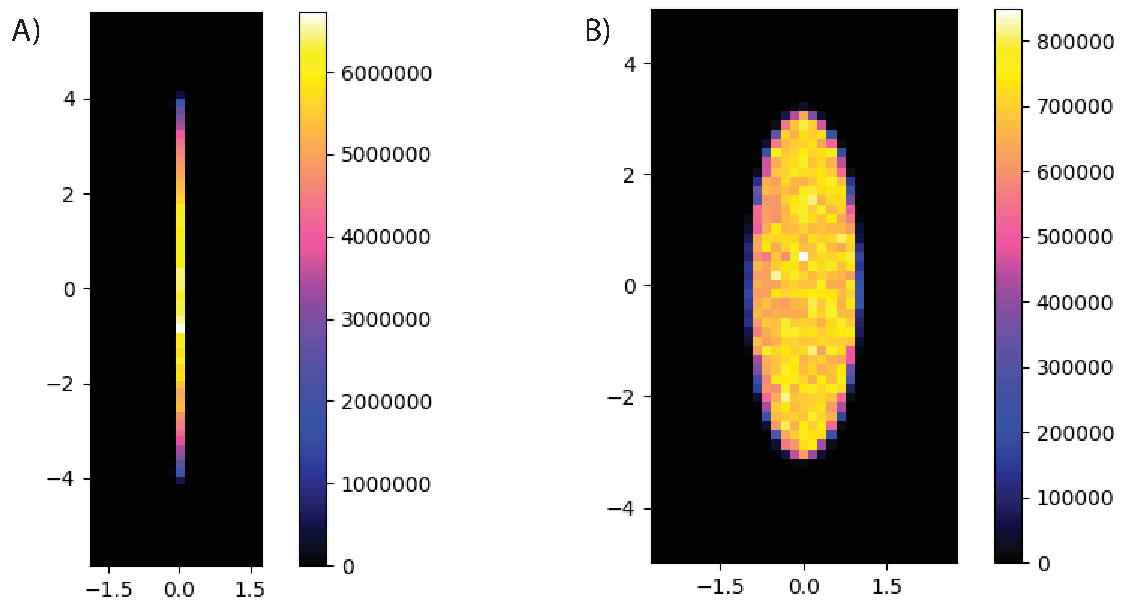
\includegraphics[width=5in]{det-pix-plot.pdf}
  \caption{
Example intensity plots. A) Results from a perfectly configured Rowland circle spectrometer. B) Same
as (A) except that the curvature of the crystal is off by 1\%. The lattice used to generate these
plots is illustrated in the Bmad manual in the \vn{Lattice Examples} chapter.
  }
\label{f:det.plot}
\end{figure}

%------------------------------------------------------------------

There is a python script for making an intensity plot of the
\vn{det_pix_out_file} in:
\begin{example}
  $ACC_ROOT_DIR/lux/scripts/plot_det_pix.py
\end{example}

The script needs python3 to run. You can invoke the script using the command:
\begin{example}
  <path-to-lux-root-dir>/scripts/plot_det_pix.py <det_pix_out_file>
\end{example}
where \vn{<det_pix_out_file>} is the actual name of the \vn{det_pix_out_file}. If the default
version of python is not python3 then the following may work
\begin{example}
  python3 <path-to-lux-root-dir>/scripts/plot_det_pix.py <det_pix_out_file>
\end{example}

The script has a number of optional arguments. The syntax for running the script is:
\begin{example}
  plot_det_pix.py \{-aspect <aspect_ratio>\} \{-scale <scale>\} 
                                         \{-plot <who_to_plot>\} \{<data_file_name>\}
  <who_to_plot> = x         # Intensity of x-polarized photons
                = y         # Intensity of y-polarized photons
                = i         # Total intensity (sum of x & y polarizations)
                = e         # Energy
  Defaults:
    <aspect_ratio>   = 1
    <scale>          = 1e3
    <data_file_name> = det_pix
    <who_to_plot>    = i
\end{example}

Figure~\ref{f:det.plot} shows two example intensity plots. 

The \vn{<scale>} parameter sets the scale of the axis numbers. A scale of \vn{1e3} results in the
axis numbers being in millimeters.

The \vn{<aspect_ratio>} parameter sets the aspect ratio of the plot. An aspect ratio of one (the
default) will mean that the vertical and horizontal scales (detector position per plotted unit
length) begin the same. An aspect ratio greater than one will enlarge the vertical scale and less than
one will enlarge the horizontal scale.

%------------------------------------------------------------------
\subsection{Other plotting}

For lattice elements like crystals or mirrors that can have a curved surface, there is a script for
drawing the surface in the directory:
\begin{example}
  util_programs/photonic_surface_plot
\end{example}
In this directory there is a \vn{README} file with documentation.

%------------------------------------------------------------------
\section{Python Scripting}
\label{s:python}

In some cases it is desired to study some output parameter while varying some input parameter. For
example, it may be desired to look at a ``rocking curve'' where the initial angle of the photons are
varied and the output intensity is monitored.  Such studies can be easily achieved using a scripting
language like \vn{python}.

Example:
\begin{listing}{1}
#!/usr/bin/env python

import subprocess
import glob

# open output file

out_file = open('output.dat', 'w')
out_file.write('#       Var         I_x/I         I_y/I   (I_x-I_y)/I           I_x           I_y             I\n')

# Loop over all runs

n_max = 10
dvar = 0.00001
for ix in range(-n_max, n_max+1):

  # Create file with var_to_change set to correct value

  var = ix * dvar
  print ('Run with my_var set to: ' + str(var))

  b_file = open ('var.bmad', 'w')
  b_file.write('my_var = ' + str(var))
  b_file.close()

  # Run lux
  # Remove any Bmad "digested" files to make sure Bmad rereads the lattice file.

  if len(glob.glob('*digested*')) > 0: subprocess.call('rm *digested*', shell=True)
  subprocess.call('/home/dcs16/linux_lib/production/bin/lux -silent', shell=True)

  # Get output

  with open('det.pix', 'r') as d_file:
    for line in d_file:
      if 'intensity_x_norm' in line: exec(line)
      if 'intensity_y_norm' in line: exec(line)
      if 'intensity_norm' in line: exec(line)

  # write results

  ii = intensity_norm
  ix = intensity_x_norm
  iy = intensity_y_norm

  if ii == 0:
    out_file.write('{:12.2e}'.format(var) + '{:14.4e}'.format(0) + 
                   '{:14.4e}'.format(0) + '{:14.4e}'.format(0))
  else:
    out_file.write('{:12.2e}'.format(var) + '{:14.4e}'.format(ix/ii) + 
                   '{:14.4e}'.format(iy/ii) + '{:14.4e}'.format((ix-iy)/ii))

  out_file.write('{:14.4e}'.format(ix) + '{:14.4e}'.format(iy) + 
                 '{:14.4e}'.format(ii) + '\n')

out_file.close()
\end{listing}

The heart of the script is the loop that begins on line 15. Each iteration of this loop creates a
file called \vn{var.bmad} (lines 22 through 24) with one line setting the variable \vn{my_var} to a
value from \vn{-n_max * dvar} to \vn{n_max * dvar} which in this case is from -10e-5 to 10e-5. The
script then runs \lux (line 30), and then extracts the pertinent data (lines 34 to 38). Finally at
the end of the loop the data is appended to the output file in lines 42 through 54.

The lattice file that \lux uses is called \vn{lat.bmad} (this is set
by the \vn{lattice_file} parameter in the \vn{lux.init} file which is
not shown). This file contains the following:
\begin{example}
  call, file = var.bmad   ! Read in my_var variable
  cryst1: crystal, ..., x_pitch = my_var
\end{example}
The \vn{my_var} variable sets the \vn{x_pitch} attribute of the
crystal named \vn{cryst1}.

To get the data after \lux is run, the script opens up a file
\vn{det.pix}. This name has been set in the \vn{lux.init} file as the
name of the \vn{det_pix_out_file} parameter:
\begin{example}
   det_pix_out_file = 'det.pix'
\end{example}
The \vn{det_pix_out_file} has a number of initial rows that give
overall parameters. Example:
\begin{example}
  master_input_file   = "lux.init"
  lattice_file        = "lat.bmad"
  normalization       =  1.000000E+02
  intensity_x_unnorm  =     9.41577E+01
  intensity_x_norm    =     9.41577E+03
  intensity_y_unnorm  =     4.64621E-02
  intensity_y_norm    =     4.64621E+00
  intensity_unnorm    =     9.42042E+01
  intensity_norm      =     9.42042E+03
\end{example}
When the script (see line 46) finds a line in \vn{det.pix} that has
the string \vn{intensity_x_norm}, the script ``executes'' this
line. The result is that the script set a variable named
\vn{intensity_x_norm} to the value given in the \vn{det.pix}
file. Similarly, the script extracts the values of
\vn{intensity_y_norm} and \vn{intensity_norm} in lines 47 and 48.

%------------------------------------------------------------------
\begin{thebibliography}{9}

\bibitem{b:bmad}
D. Sagan,
"Bmad: A Relativistic Charged Particle Simulation Library"
Nuc.\ Instrum.\ \& Methods Phys.\ Res.\ A, {\bf 558}, pp 356-59 (2006).

\end{thebibliography}
\end{document}  
